\documentclass[../main.tex]{subfiles}

\begin{document}
The CHIPS Architecture allows for many different dies to be connected post-silicon. For dies to be connected post-silicon, there need to be both a physical layer and protocol layer. These two layers make up the SOC. The chips sub-system is comprised of a control unit (Rocket Core), off and on chip memory controllers and two accelerators.
\subsection{CHIPS SOC}
CHIPS physical layer allow die to die commutation over an interposer. This layer use set of 40bit AIB Channels. Groups of these 40bit channels makeup the protocol layer. The protocol layer is make up of three bus, off-chip bus (CIPI protocol), Mbus (AXI4 protocol) and XBus (AXI4 protocol). The Mbus is an AXI4 cross-point that connects Rocket Core and accelerators to on-chip and off-chip memory. The Xbus is a AXI4 corss-point that connects the Rocket Core to the accelerators. This bus is used to interface with accelerators. The off-chip Bus allow for a bigger memory space and in turn run a bigger workload.
\subsubsection{Physical Layer}
AIB is a specialized driver that allows signals to be driven form one die through interposer and up into another die. AIB allows for tri-state signals. In this Architecture, AIB was configured to transmit or receive. An AIB channel includes 8 bits for clock and 40 bits for data transfer. 
\subsubsection{Protocol Layer}
The Protocol Layer is consist of two different protocols, AXI and CIPI. AXI is a protocol that allows for point to point data transfer. All transfer are master initiated. On the Mbus, the Rocket Core and accelerators initiate the data transfer. On the Xbus, the Rocket Core initiate data transfer. 
\subsection{Rocket Core RISC-V Processor}
\begin{figure}[H]
    \centering
    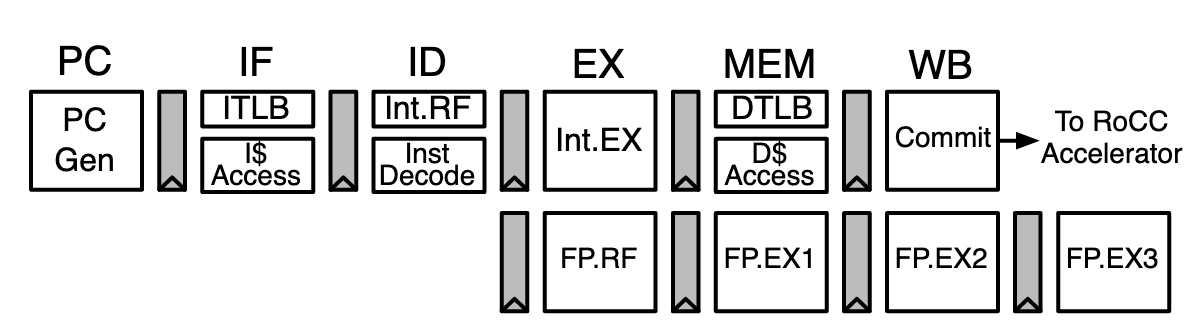
\includegraphics[scale=.4]{pngs/RocketPipeline.png}
    \caption{Rocket Chkp Pipeline\cite{Asanović:EECS-2016-17}}
    \label{fig:RocketChipPipeline}
\end{figure}
The Rocket Core is a in-order scalar RISC-V processor. It was developed at UC Berkeley. The Rocket Core is 
\subsection{Chips Accelerators}
\subsubsection{LSTM}
\blindtext
\subsubsection{SCNN}
\blindtext
\end{document}

